%%%%%%%%%%%%%%%%%%%%%%%%%%%%%%%%%%%%%%%%%
% Thin Sectioned Essay
% LaTeX Template
% Version 1.0 (3/8/13)
%
% This template has been downloaded from:
% http://www.LaTeXTemplates.com
%
% Original Author:
% Nicolas Diaz (nsdiaz@uc.cl) with extensive modifications by:
% Vel (vel@latextemplates.com)
%
% License:
% CC BY-NC-SA 3.0 (http://creativecommons.org/licenses/by-nc-sa/3.0/)
%
%%%%%%%%%%%%%%%%%%%%%%%%%%%%%%%%%%%%%%%%%

%----------------------------------------------------------------------------------------
%	PACKAGES AND OTHER DOCUMENT CONFIGURATIONS
%----------------------------------------------------------------------------------------

\documentclass[a4paper, 12pt]{article} % Font size (can be 10pt, 11pt or 12pt) and paper size (remove a4paper for US letter paper)

\usepackage[protrusion=true,expansion=true]{microtype} % Better typography
\usepackage{graphicx} % Required for including pictures
\usepackage{wrapfig} % Allows in-line images
\usepackage{caption}
\usepackage{amsmath}
\usepackage{mathtools}
\usepackage{float}
\usepackage{mathpazo} % Use the Palatino font
\usepackage[T1]{fontenc} % Required for accented characters
\linespread{1.05} % Change line spacing here, Palatino benefits from a slight increase by default

\makeatletter
\renewcommand\@biblabel[1]{\textbf{#1.}} % Change the square brackets for each bibliography item from '[1]' to '1.'
\renewcommand{\@listI}{\itemsep=0pt} % Reduce the space between items in the itemize and enumerate environments and the bibliography

\renewcommand{\maketitle}{ % Customize the title - do not edit title and author name here, see the TITLE block below
\begin{flushright} % Right align
{\LARGE\@title} % Increase the font size of the title

\vspace{50pt} % Some vertical space between the title and author name

{\large\@author} % Author name
\\\@date % Date

\vspace{40pt} % Some vertical space between the author block and abstract
\end{flushright}
}

%----------------------------------------------------------------------------------------
%	TITLE
%----------------------------------------------------------------------------------------

\title{\textbf{\'Atomo de Hidrogeno relativista}\\ % Title
La perspectiva de Dirac} % Subtitle

\author{\textsc{Juan David Orjuela Zu\~niga \\ Juan Nicol\'as Garavito Camargo} % Author
\\{\textit{Departamento de F\'isica\\}
\textit{Universidad de los Andes, Bogot\'a, Colombia}}} % Institution

\date{\today} % Date

%----------------------------------------------------------------------------------------

\begin{document}

\maketitle % Print the title section

%----------------------------------------------------------------------------------------
%	ABSTRACT AND KEYWORDS
%----------------------------------------------------------------------------------------

%\renewcommand{\abstractname}{Summary} % Uncomment to change the name of the abstract to something else

\begin{abstract}
Resumen, JD \& JN
\end{abstract}
\hspace*{3,6mm}\textit{Keywords:}  % Keywords

\vspace{30pt} % Some vertical space between the abstract and first section

%----------------------------------------------------------------------------------------
%	ESSAY BODY
%----------------------------------------------------------------------------------------

\section{Antecedentes historicos}
JD

% ------------------------------------- Ecuacion de Dirac --------------------------------------
\section{Ecuaci\'on de Dirac}
La ecuaci\'on de Dirac al igual que la ecuaci\'on de Klain-Gordon es una 
ecuaci\'on relativista de la mec\'anica cuantica. Adem\'as tiene en cuenta
part\'iculas de sp\'in $s=1/2$ tales como electrones, protones, neutrones etc. 

A continuaci\'on de se derivara la ecuaci\'on de Dirac mediante argumentos
de simetr\'ia (mostrando as\'i una manera alternativa a la vista en clase). 
Una ecuaci\'on relativista debe ser simetrica tanto en el tiempo como en el 
espacio, esto debido a que el tiempo y el espacio son una misma cantidad 
en las transformaciones de Lorentz.

Es sabido de relatividad especial que la energ\'ia de una part\'icual esta dada
por:

\begin{equation}
E^2 = m^2c^4 + p^2c^2
\end{equation}

Si expresamos $E$ y $p$ como operadores obtenemos la ecuaci\'on de Klein-Gordon:

\begin{equation}
\left( \nabla^2 - \dfrac{1}{c^2}\dfrac{\partial^2}{\partial t^2} - \dfrac{m^2c^2}{\hbar^2}   \right)\psi(\mathbf{r}, t) = 0
\end{equation} 


\begin{equation}\label{eq:dirac1}
\dfrac{1}{c}\dfrac{\partial \psi_i(\mathbf{r},t)}{\partial t} =
- \sum \limits_{k=x,y,z} \sum \limits_{n=1}^{N}\alpha^k_{i,n} \dfrac{\partial \psi_n}{\partial k} -
\dfrac{imc}{\hbar}\sum \limits_{n=1}^{N}\beta_{i,n}\psi_n(\mathbf{r}, t)
\end{equation}

Donde el primer termino del lado derecho corrsponde a la contribucion 
de todas las derivadas espaciales de todas las componentes de la funci\'on 
de onda y el segundo termino es una combinacion lineal de todas las 
componentes de $\psi$. $\alpha$ y $\beta$ son constantes que hacen que la 
ecuaci\'on tenga las dimensiones correctas. (\ref{eq:dirac1}) puede escribirse
de forma matricial haciendo la suma de todas las componentes $N$.   

\begin{equation}
i\hbar \partial_t \psi(\mathbf{r},t) = \hat{\mathbf{H}}\psi(\mathbf{r},t) =
(c\widetilde{\alpha}\cdot \hat{\mathbf{p}} + \widetilde{\beta}mc^2)\psi(\mathbf{r},t)
\end{equation}

Donde $\partial_t = \partial / \partial t$ y $\widetilde{\alpha}$ y $\widetilde{\beta}$ son matrices de dimension $N$, y se llaman \textbf{matrices de Dirac}.
Como se vio en clase estas matrices deben satisfacer las siguientes condiciones:\\

\[
\alpha_i^2 = \beta^2 = I \\
\]
\[
\alpha \beta + \beta \alpha = 0 \\
\]
\[
\alpha_j \alpha_i + \alpha_i \alpha_j = 0
\]
\[
i,j=x, y, z\\
\] 

Las matrices que cumplen con estas condiciones para $N=4$ estan definidas en terminos
de las matrices de Pauli:

\begin{equation}
\widetilde{\alpha_i}=
\begin{pmatrix}
0 & \widetilde{\sigma_i}\\
\widetilde{\sigma_i} & 0 \\
\end{pmatrix}
\end{equation}

\begin{equation}
\widetilde{\beta}=
\begin{pmatrix}
\widetilde{\mathbf{I_2}} & 0\\
0 & -\widetilde{\mathbf{I_2}} \\
\end{pmatrix}
\end{equation}

Donde $\widetilde{\mathbf{I_2}}$ son matrices unitarias de dimension 2. 
Adicionalmente las matrices de \textbf{spin} de Pauli de 4 dimensiones
estan definidas como:

\begin{equation}
\widetilde{\sigma_{4i}}=
\begin{pmatrix}
\widetilde{\sigma_i} & 0 \\
0 & \widetilde{\sigma_i}  \\
\end{pmatrix}
\end{equation}

Las matrices $\alpha$, $\beta$ y $\sigma$ cumplen con las siguientes relaciones:

\[
\widetilde{\sigma_i}^2 = \widetilde{\mathbf{I}}
\]

\[
[\widetilde{\sigma_i}, \widetilde{\sigma_j}] = 2i\epsilon_{ijk}\widetilde{\sigma_k}
\]

\[
\{\widetilde{\sigma_i},\widetilde{\sigma_j}\} = 2\widetilde{\mathbf{I}}\delta_{ij}
\]

\[
[\widetilde{\sigma_i}, \widetilde{\alpha_i}] = 0
\]

\[
\{ \widetilde{\sigma_i}, \widetilde{\alpha_j} \} = 0 \ i \neq j
\]

\[
\widetilde{\alpha} \times \widetilde{\alpha} = 2i\widetilde{\sigma}
\]

\[
\widetilde{\gamma}_i = \widetilde{\beta}\widetilde{\alpha}_i = 
\begin{pmatrix}
0 & \widetilde{\sigma}_i \\
-\widetilde{\sigma}_i & 0 \\
\end{pmatrix}
\]

Donde $i = x, y, z$. 


\[
\widetilde{\gamma}_4 = \widetilde{\beta}\widetilde{I} = 
\begin{pmatrix}
\widetilde{I} & 0 \\
0 & -\widetilde{I}  \\
\end{pmatrix}
\]

\begin{equation}\label{eq:gamma5}
\widetilde{\gamma}_5 = i\widetilde{\gamma}_1 \widetilde{\gamma}_2 \widetilde{\gamma}_3 \widetilde{\gamma}_4 = 
\begin{pmatrix}
0 & -\widetilde{I} \\
-\widetilde{I} & 0 \\
\end{pmatrix}
\end{equation}

%----------------------- Solucion de el atomo de hidrogeno con Dirac -------------------------

\section{Soluci\'on de la ecuaci\'on de Dirac para el \'atomo de Hidrogeno}

%----------Coordenadas radiales-----------------------

\subsection{Ecuaci\'on de Dirac en coordenadas esfericas}

La ecuaci\'on de Dirac para un potencial radial $V(r)$ es:

\begin{equation}\label{eq:diracvr}
(c \widetilde{\alpha} \cdot \hat{p} + \widetilde{\beta} m c^2 + V(r) ) \phi(r) = E \phi (r)
\end{equation}

En (\ref{eq:diracvr}) el termino que se debe transformar a coordenadas radiales
 es $\widetilde{\alpha} \cdot \hat{\mathbf{p}}$, ya que \textbf{$\beta$} es independiente del 
sistema de coordenadas. 

\begin{equation}\label{eq:alphap}
\widetilde{\alpha} \cdot \hat{\mathbf{p}} = -i \hbar \widetilde{\alpha} \cdot \nabla
\end{equation}

Haciendo uso de la identidad vectorial: 

\begin{equation}\label{eq:identity}
\nabla = \hat{\mathbf{r}}(\hat{\mathbf{r}}\cdot \nabla) - \hat{\mathbf{r}} \times (\hat{\mathbf{r}} \times \nabla)  
\end{equation}

Teniendo en cuenta la simetr\'ia esferica del sistema, es decir donde $\partial/\partial \theta = 0$
y $\partial/\partial \phi = 0$  (\ref{eq:identity}) se puede expresar:

\begin{equation}\label{eq:nabla1}
\mathbf\nabla = \hat{\mathbf{r}}(\dfrac{\partial}{\partial r}) - \hat{\mathbf{r}} \times (\hat{\mathbf{r}} \times \nabla)
\end{equation}

El segundo termino en \ref{eq:nabla1} se puede expresar en terminos del momento angular $\mathbf{L} = -i\hbar \mathbf{r} \times \mathbf{\nabla}$.

\begin{equation}\label{eq:nabla}
\mathbf{\nabla} =  \hat{\mathbf{r}}(\dfrac{\partial}{\partial r}) - \dfrac{i}{\hbar}\dfrac{\hat{\mathbf{r}}}{r} \times \mathbf{L}
\end{equation}

Por lo tanto \ref{eq:alphap} se puede escribir en terminos de (\ref{eq:nabla}) como:

\begin{equation}\label{eq:alphap2}
\widetilde{\alpha}\cdot \mathbf{\hat{p}} = -i\hbar \widetilde({\alpha}\cdot \hat{\mathbf{r}}(\dfrac{\partial}{\partial r}) - 
\dfrac{i}{\hbar}\widetilde{\alpha}\cdot \dfrac{\hat{\mathbf{r}}}{r} \times \mathbf{L})
\end{equation}

El \'ultimo termino de (\ref{eq:alphap2}) se puede expresar como:

\begin{equation}\label{eq:prop1}
\widetilde{\alpha}\cdot\hat{\mathbf{r}}\widetilde{\alpha} \cdot \hat{\mathbf{L}} = i\widetilde{\sigma}\cdot \hat{\mathbf{r}} \times \mathbf{L}
\end{equation}

En donde se uso la relaci\'on:

\begin{equation}
\widetilde{\alpha}\cdot \hat{\mathbf{r}}\widetilde{\alpha}\cdot \hat{\mathbf{L}}
= i \widetilde{\sigma}\cdot \hat{\mathbf{r}}\times \hat{\mathbf{L}}
\end{equation}

(Ver la demonstraci\'on de esta propiedad en \S \ref{sec:apendice}), multiplicando a ambos lados de (\ref{eq:prop1}) por $\gamma_5$ (ver \S \ref{sec:gamma5}) 
obtenemos:   

\begin{equation}
i\widetilde{\alpha}\cdot\hat{\mathbf{r}}\widetilde{\sigma} \cdot \hat{\mathbf{L}} = -\widetilde{\alpha}\cdot \hat{\mathbf{r}} \times \mathbf{L}
\end{equation}

Por lo tanto \ref{eq:alphap2} se puede escribir como:

\begin{equation}\label{eq:alphap3}
\widetilde{\alpha}\cdot \mathbf{\hat{p}} = -i\hbar \widetilde{\alpha}\cdot \hat{\mathbf{r}}\partial_r + \dfrac{i}{|\mathbf{r}|}
\widetilde{\alpha}\cdot \hat{\mathbf{r}}\widetilde{\sigma}\cdot \hat{\mathbf{L}}
\end{equation} 

Finalmente escribiendo el ultimo termino de (\ref{eq:alphap3}) en terminos
del vector $\hat{K}$ (Ver pasos intermedios en \S \ref{sec:k}) se obtiene:

\begin{equation}\label{alphap4}
\widetilde{\alpha} \cdot \mathbf{\hat{p}} = -i\hbar \widetilde{\alpha}\cdot \hat{\mathbf{r}}\partial_r + \dfrac{i}{|\mathbf{r}|} \widetilde{\alpha_r}(\widetilde{\beta}\hat{K}-\hbar)
\end{equation}

En \ref{eq:diracvr}, por tanto la ecuaci\'on de Dirac en coordenadas esfericas
es:

\begin{equation}
\left (ic\widetilde{\gamma_5}\widetilde{\sigma_r} \left (\hbar \partial_r + \dfrac{\hbar}{r} -  \dfrac{\widetilde{\beta}\hat{K}}{r}\right )  + \widetilde{\beta} m c^2 + V(r) \right ) \phi(r) = E \phi (r)
\end{equation}


Vamos entonces a insistir que nuestro autoestado de 4 componentes sea lo m\'as parecido posible a los espinores de dos componentes de Pauli:

\begin{equation}
\phi^{m_j}_{\kappa} (\vec{r} ) = \left( \substack{g_{\kappa}(r)\chi^{m_j}_\kappa (\hat{r}) \\ if_\kappa(r)\chi^{m_j}_{-\kappa} (\hat{r}) } \right) 
\end{equation}

\begin{equation}
-c \hbar  \left( \frac{\partial}{\partial r}+\frac{1}{r}+\frac{\kappa}{r} \right) g_{\kappa}(r)\chi^{m_j}_{-\kappa} +(E-V(r)+mc^2)f_{\kappa}(r)\chi^{m_j}_{-\kappa}
\end{equation}


\begin{equation}
c \hbar  \left( \frac{\partial}{\partial r}+\frac{1}{r}+\frac{\kappa}{r} \right) f_{\kappa}(r)\chi^{m_j}_{\kappa} +(E-V(r)-mc^2)g_{\kappa}(r)\chi^{m_j}_{\kappa}
\end{equation}


lo que permite cancelar el t\'ermino $\chi^{m_j}_{\kappa}$ y ver que el imaginario puro de las soluciones tiene el papel de asegurar que la parte radial de la autofunci\'on es real. Se pueden reescribir entonces como


\begin{equation}
\frac{\partial g_{\kappa}(r)}{\partial r} =\frac{\kappa+1}{r}g_{\kappa}(r)+\frac{1}{c\hbar}(E-V(r)+mc^2)f_{\kappa}(r)
\end{equation}

\begin{equation}
\frac{\partial f_{\kappa}(r)}{\partial r} =\frac{\kappa-1}{r}f_{\kappa}(r)-\frac{1}{c\hbar}(E-V(r)-mc^2)g_{\kappa}(r)
\end{equation}

Que es la forma usual de la ecuaci\'on de radial de Dirac. Sin embargo, a menudo es \'util hacer los reemplazos $u_{\kappa}(r)=rg_{\kappa}(r)$ y $v_{\kappa}(r)=rg_{\kappa}(r)$, lo que permite que la ecuaci\'on se vea as\'i


\begin{equation}
\frac{\partial u_{\kappa}(r)}{\partial r} =-\frac{\kappa}{r}u_{\kappa}(r)+\frac{1}{c\hbar}(E-V(r)+mc^2)v_{\kappa}(r)
\end{equation}

\begin{equation}
\frac{\partial v_{\kappa}(r)}{\partial r} =\frac{\kappa}{r}v_{\kappa}(r)+\frac{1}{c\hbar}(E-V(r)-mc^2)u_{\kappa}(r)
\end{equation}

Que tambi\'en es una forma v\'alida de la ecuaci\'on de Dirac. Para el \'atomo de Hidrogeno el potencial
tiene la forma:

\begin{equation}
V(r) = - \dfrac{Ze^2}{4\pi \eps r}
\end{equation}

Para simplificar 

\begin{equation}\label{eq:phi1}
\phi_1(\rho) = \rho^s \sum \limits_{m=0}^{\infty} a_m \rho^m
\end{equation}


\begin{equation} \label{eq:phi2}
\phi_2(\rho) = \rho^s \sum \limits_{m=0}^{\infty} b_m \rho^m
\end{equation}

Donde los coeficientes $a_m$ y $b_m$ estan definidos como (El lector interesado 
puedo ver el desarrollo detallado en el ap\'endice):

\begin{equation}
a_m = (-1)^m \dfrac{(n'-1)(n'-2)\cdot\cdot\cdot(n'-m)}{m!(2s+1)(2s+2)\cdot\cdot\cdot(2s+m)}a_0
\end{equation}

\begin{equation}
b_m = (-1)^m \dfrac{n'(n'-1)\cdot\cdot\cdot(n'-m+1)}{m!(2s+1)(2s+2)\cdot\cdot\cdot(2s+m)}b_0
\end{equation}

\begin{equation}
b_0 = -\dfrac{\kappa - \xi k_c /\lambda}{n'}a_0
\end{equation}

Donde $n' = W_c\xi/\lambda - s$. Reemplazando $a_m$ y $b_m$ en las ecuaciones (\ref{eq:phi1}) y (\ref{eq:phi2})
podemos expresar como:

\[
\phi_1(\rho) = \rho^s a_0 \sum  \limits_{m=0}^{\infty} (-1)^m \dfrac{(n'-1)(n'-2)\cdot\cdot\cdot(n'-m)}{m!(2s+1)(2s+2)\cdot\cdot\cdot(2s+m)}a_0 \rho^m 
\]

\[
\phi_1(\rho) = \rho^s a_0 \left( \dfrac{(1-n')}{2s+1} \rho + \dfrac{(1-n')(2-n')\rho^2}{(2s+1)(2s+2)}\dfrac{\rho^2}{1!} + \cdot\cdot\cdot  \right)
\]

\begin{equation}\label{eq:sol1}
\phi_1(\rho) = 	\rho^s a_0 M(1-n',2s+1,\rho)
\end{equation}

Donde $M$ es la funcion hipergeometrica. De manera an\'aloga para $\phi_2(\rho)$ obtenemos:

\begin{equation}\label{eq:sol2}
\phi_2(\rho) = \rho^s b_0 M(-n',2s+1,\rho) = \rho^s \dfrac{\kappa - \xi kc / \lambda}{n'} a_0 M(-n',2s+1,\rho)
\end{equation}

Aplicando condiciones de frontera podemos encontrar los valores permitidos para $a_0$, las soluciones
(\ref{eq:sol1}) y (\ref{eq:sol2}) deben converger para $r \rightarrow \infty$. El comportamiento 
asint\'otico de (\ref{eq:sol2}) y de (\ref{eq:sol1}) se puede ver en la Fig.\ref{fig:hypgeo}, 
en donde para valores negativos de $n'$ y $2s-1$ las funciones no convergen.

\begin{figure}
\centering
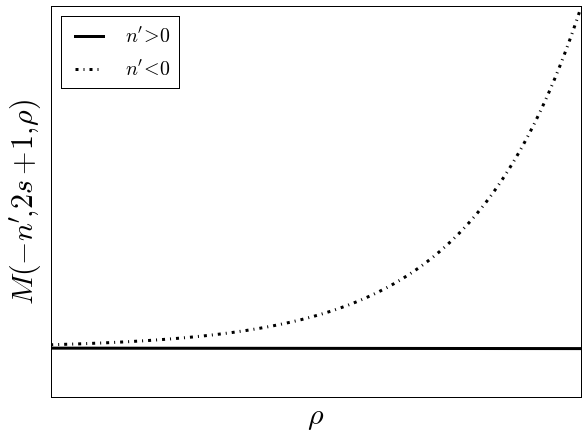
\includegraphics[scale=0.4]{hypgeo.png}
\caption*{Comportamiento asint\'otico de la funci\'on hipergeometrica.
\label{fig:hypgeo}}
\end{figure}  

Para $n' = 0$ la funci\'on hipergeometrica converge pero las funciones (\ref{eq:sol2}) y (\ref{eq:sol1})
divergen. Por lo tanto si $n'=0$ la constante $a_0 = 0$ para (\ref{eq:sol1}) y $\kappa - \xi kc / \lambda$
para (\ref{eq:sol2}), lo cual implica que para $n'=0$ $\kappa > 0$. 

\section{Ap\'endice: Demostraci\'ones y desarrollos matematicos}\label{sec:apendice}

\subsection{Propiedades de las matrices $\widetilde{\gamma}$}\label{sec:gamma5}

\[
\widetilde{\gamma_5} = 
\begin{pmatrix} 
0 & - \widetilde{I} \\
-\widetilde{I} & 0 \\
\end{pmatrix}
\]

Donde $\widetilde{I}$ es la matriz identidad de dos dimensiones. Operando  $\widetilde{I}$ 
en $\widetilde{\alpha}$ y $\widetilde{\sigma}$ obtenemos:

\[
\widetilde{\gamma_5}\widetilde{\alpha_i} = 
\begin{pmatrix} 
0 & - \widetilde{I} \\
-\widetilde{I} & 0 \\
\end{pmatrix} 
\begin{pmatrix} 
0 & \sigma_i \\
\sigma_i & 0 \\
\end{pmatrix} 
= 
\begin{pmatrix}
-\sigma_i & 0 \\
0 & -\sigma_i
\end{pmatrix}
= -\widetilde{\sigma_i}
\]

y an\'alogamente:

\[
\widetilde{\gamma_5}\widetilde{\sigma_i} = 
\begin{pmatrix} 
0 & - \widetilde{I} \\
-\widetilde{I} & 0 \\
\end{pmatrix} 
\begin{pmatrix} 
\sigma_i & 0 \\
0 & \sigma_i  \\
\end{pmatrix} 
= 
\begin{pmatrix}
0 & -\sigma_i \\
-\sigma_i & 0 \\
\end{pmatrix}
= -\widetilde{\alpha_i}
\]

Adicionalmente las matrices $\widetilde{\gamma}$ cumplen con las siguientes
propiedades de conmutaci\'on y anticonmutaci\'on:

\[
\{ \widetilde{\gamma}_i, \widetilde{\gamma}_j \} = 0 \ i \neq j
\]

Y $\widetilde{\gamma}_5$ conmuta con $\widetilde{\alpha}_i$ y $\widetilde{\sigma}_i$: 

\[
[\widetilde{\gamma}_5, \widetilde{\alpha}_i] = [\widetilde{\gamma}_5,\widetilde{\sigma}_i] = 0
\]

\subsection{Definici\'on del operador $\hat{K}$}\label{sec:k}

\begin{equation}
\widetilde{\hat{K}} = \widetilde{\hat{L}}\cdot \widetilde{\sigma} + \hbar
\end{equation}

Con autovalor $-\hbar \kappa$ y donde $\kappa$ puede tomar los siguientes
valores:

\[ \kappa = 
\begin{cases}
-l - 1 \rightarrow j = l + 1/2  \\
l \rightarrow j = l - 1/2 \\ 
\end{cases}
\]  

% ---------------- coeficientes a_m y b_m

\subsection{Derivaci\'on de los coeficientes $a_m$ y $b_m$}

\begin{equation}\label{eq:am}
a_m(m+s) = a_{m-1} - \dfrac{Wc\xi}{\lambda}a_m - \left(\kappa + \dfrac{\xi kc}{\lambda}\right) b_m
\end{equation}

\begin{equation}\label{eq:bm}
b_m(m+s) = \left( -\kappa + \dfrac{\xi kc}{\lambda}  \right)a_m + \dfrac{Wc \xi}{\lambda}b_m
\end{equation}

Para poder estudiar bien estas relaciones veamos el caso $m=0$ que implica que $a_{m-1}$. Este 
sistema de ecuaciones tendr\'a soluciones si el determinante de los coeficientes es diferente de
cero. 

\[
\begin{vmatrix}
s + Wc \xi/\lambda & \kappa + \xi kc/\lambda \\
\kappa - \xi kc/lambda & s-Wc \xi/lambda \\
\end{vmatrix}
= 0
\]

Lo que implica que:

\[
s^2 - \dfrac{Wc^2 \xi^2}{\lambda^2} = \kappa^2 - \dfrac{\xi^2 kc^2}{\lambda^2}
\]

Y recordando que $\lambda^2 = kc^2 + Wc^2$ se obtiene:

\[
s = \pm \sqrt{\kappa^2 - \xi^2}
\]

Siempre se escoge el signo positivo en la soluci\'on de $s$ debido a que se debe garantizar siempre
que las ecuaciones (\ref{eq:phi1})  y (\ref{eq:phi2}) sean cuadrado integrables. Es de interes entonces
encontrar las relaciones de recurrencia para $a_m$ y $b_m$, por lo tanto se despeja $b_m/a_m$ de (\ref{eq:bm})

\begin{equation}\label{eq:ambm}
\dfrac{b_m}{a_m} = \dfrac{\kappa - \xi kc/\lambda}{Wc\xi /\lambda - m - s} = \dfrac{\kappa - \xi kc/\lambda}{n'-m}
\end{equation} 

En donde se definio $n' = Wc \xi /\lambda - s$. Reemplazando (\ref{eq:ambm}) en (\ref{eq:am}) se obtiene:

\begin{equation}\label{eq:am-1}
a_m = - \dfrac{n-m}{m(2s+m)}a_{m-1}
\end{equation} 

Que para el caso de $m=0$ se obtiene:

\begin{equation}
b_0 = \dfrac{\kappa - \xi kc/\lambda}{n'}a_0
\end{equation}

De (\ref{eq:am-1}) se puede ver que la relacion de recurrencia para $a_m$ es:

\begin{equation}
a_m = (-1)^m \dfrac{(n'-1)(n'-2)\cdot\cdot\cdot(n'-m)}{m!(2s+1)(2s+2)\cdot\cdot\cdot(2s+m)}a_0
\end{equation} 

Y con un proceidimiento an\'alogo se deduce que $b_m$ es:
 
\begin{equation}
b_m = (-1)^m \dfrac{n'(n'-1)\cdot\cdot\cdot (n'-m +1)}{m!(2s+1)(2s+2)\cdot\cdot\cdot(2s+m)}b_0
\end{equation}

%	BIBLIOGRAPHY
%----------------------------------------------------------------------------------------

\bibliographystyle{unsrt}

\bibliography{bibliografia}

%----------------------------------------------------------------------------------------

\end{document}
